\documentclass[12pt,titlepage]{article}
\usepackage[margin=1.25in]{geometry}
\usepackage{graphicx,amsmath,blindtext,minted}
\usepackage{pgf-umlcd}

%% Variables definition
\newcommand{\vSubject}{Data Structure and Algorithm Practicum}
\newcommand{\vSubtitle}{Class and Object}
\newcommand{\vName}{Dicha Zelianivan Arkana}
\newcommand{\vNIM}{2241720002}
\newcommand{\vClass}{1i}
\newcommand{\vDepartment}{Information Technology}
\newcommand{\vStudyProgram}{D4 Informatics Engineering}

%% [START] Tikz related stuff
\usepackage{tikz}
\usetikzlibrary{svg.path,calc,shapes.geometric,shapes.misc}
\tikzstyle{terminator} = [rectangle, draw, text centered, rounded corners = 1em, minimum height=2em]
\tikzstyle{preparation} = [chamfered rectangle, chamfered rectangle sep=0.75em, draw, text centered, minimum height = 2em]
\tikzstyle{process} = [rectangle, draw, text centered, minimum height=2em]
\tikzstyle{decision} = [diamond, aspect=2, draw, text centered, minimum height=2em]
\tikzstyle{data}=[trapezium, draw, text centered, trapezium left angle=60, trapezium right angle=120, minimum height=2em]
\tikzstyle{connector} = [line width=0.25mm,->]
%% [END] Tikz related stuff

%% [START] Fancy header related stuff
\usepackage{fancyhdr}
\pagestyle{fancy}
\setlength{\headheight}{15pt} % compensate fancyhdr style
\fancyhead{}
\fancyfoot{}
\fancyfoot[L]{\thepage}
\fancyfoot[R]{\textit{\vSubject - \vSubtitle}}
\renewcommand{\footrulewidth}{0.4pt}% default is 0pt, overline for footer
%% [END] Fancy header related stuff

%% [START] Custom tabular command related stuff
\usepackage{tabularx}
\newcommand{\details}[2]{
    #1 & #2  \\
}
%% [END] Custom tabular command related stuff

%% [START] Figure related stuff
\newcommand{\image}[3][1]{
    \begin{figure}[h]
        \centering
        \includegraphics[#1]{#2}
        \caption{#3}
        \label{#3}
    \end{figure}
}
%% [END] Figure related stuff

\begin{document}
\begin{titlepage}
    \centering
    \vfill
    {\bfseries\LARGE
        \vSubject\\
        \vskip0.25cm
        \vSubtitle
    }
    \vfill
    \includegraphics[width=6cm]{images/polinema-logo.png}
    \vfill
    {
        \textbf{Name}\\
        \vName\\
        \vskip0.5cm
        \textbf{NIM}\\
        \vNIM\\
        \vskip0.5cm
        \textbf{Class}\\
        \vClass\\
        \vskip0.5cm
        \textbf{Department}\\
        \vDepartment\\
        \vskip0.5cm
        \textbf{Study Program}\\
        \vStudyProgram
    }
\end{titlepage}

\section{Question}
\begin{enumerate}
    \item {
        Mention 2 characteristics of class/object!

        \begin{itemize}
            \item They have data (attributes)
            \item They have behaviours (methods)
            \item 
        \end{itemize}
    }
    \item {
        What is the keyword used to declare a class?

        In Java, we can use the \texttt{class} keyword to define a class
    }
    \item {
        In the class \textbf{Barang} at the \textbf{Part 2}, how many attributes owned by that class? What are they?

        There are 4 attributes in class \textbf{Barang} from \textbf{Part 2} which are:
        \begin{itemize}
            \item \texttt{String namaBarang}
            \item \texttt{String jenisBarang}
            \item \texttt{int stok}
            \item \texttt{int hargaSatuan}
        \end{itemize}
    }
    \item {
        In the class \textbf{Barang} at the \textbf{Part 2}, on which line of code are the attributes declared?

        \begin{itemize}
            \item \texttt{String namaBarang} - Line 4
            \item \texttt{String jenisBarang} - Line 4
            \item \texttt{int stok} - Line 5
            \item \texttt{int hargaSatuan} - Line 5
        \end{itemize}
    }
    \item {
        In the class \textbf{Barang} at the \textbf{Part 2}, how many methods owned by that class? What are they?

        \begin{itemize}
            \item \texttt{void tampilBarang()}
            \item \texttt{void tambahStok(int n)}
            \item \texttt{void tampilBarang(int n)}
            \item \texttt{int hitungHargaTotal(int jumlah)}
        \end{itemize}
    }
    \newpage
    \item {
        In the class \textbf{Barang} at the \textbf{Part 2}, on which line of code are the methods declared?

        \begin{itemize}
            \item \texttt{void tampilBarang()} - Line 7
            \item \texttt{void tambahStok(int n)} - Line 13
            \item \texttt{void tampilBarang(int n)} - Line 16
            \item \texttt{int hitungHargaTotal(int jumlah)} - Line 19
        \end{itemize}
    }
    \item {
        In the method \texttt{kurangiStok()} in class \textbf{Barang}, modify the method so that it will check the availability of \textbf{stok} before subtracting the \textbf{stok}!
        Then it will not be any subtraction if the \textbf{stok} is already less then or equals to zero.

        \begin{minted}[autogobble,fontsize=\small]{java}
            void kurangiStok(int n) {
                if (stok < n) return;
                stok = stok - n;
            }
        \end{minted}
    }
    \item {
        Please give your explanation, why is the method \textbf{tambahStok()} created with an \texttt{int} parameter?
        What is the use of that parameter in that method?

        The parameter \texttt{(int n)} will be used to add the stock of the goods.
        The int data type is used because we store the stock in \texttt{int},
        if we use other datatype such as \texttt{double} or \texttt{float} then we need to also adjust the parameter, or type cast it. 
    }
    \item {
        Why does method \textbf{hitungHargaTotal()} have a non-void (int) data type? What is it for?

        We use a non-void, in this case an \texttt{int},
        because we want to receive the total price of the goods from the caller, in this case the caller is the main method.
    }
    \item {
        Why does the method \textbf{tambahStok()} have void data type?

        Because we only need to add the goods stock, we don't need to receive the stock amount from the caller.
    }
    \item {
        In class \textbf{BarangMain}, in \textbf{Part 3}, on which line of code does the instantiation process run? and what is the name of the resulting object?

        The class \textbf{Barang} is instantiated in the 5th line and the object is called \textbf{b1}.
    }
    \newpage
    \item {
        How do you access the attributes and methods of the objects?

        We can use the dot notation on the instance of the class.
        For example, if we have a property called \texttt{stock}, a method called \texttt{void addStock(int n)},s and an object called \texttt{good},
        we can do it like this:

        \begin{minted}[autogobble,fontsize=\small]{java}
            Good good = new Good();
            good.addStock(10); // accessing the method
            System.out.println(good.stock); // accessing the attribute
        \end{minted}
    }
    \item {
        In class \textbf{Barang} in \textbf{Part 4}, on which line of code is the parametric constructor declared?

        The parametric constructor is declared in Line 9 through Line 14
    }
    \item {
        In class \textbf{Barang} in \textbf{Part 4}, what does actually we do on line of code 16?

        On the 16th line, we define a method to show the goods detail.
    }
    \item {
        Try to create another object called \textbf{b3} from class \textbf{Barang} by using the parametric constructor of class \textbf{Barang}

        \begin{minted}[autogobble,fontsize=\small]{java}
            Barang b3 = new Barang("QK65", "Mechanical Keyboard", 5_800_000, 10);
        \end{minted}
    }
\end{enumerate}

\renewcommand{\umldrawcolor}{black}
\renewcommand{\umlfillcolor}{white}

\newpage

\section{Task}
\begin{enumerate}
    \item {
        Create the program based on the class diagram below!

        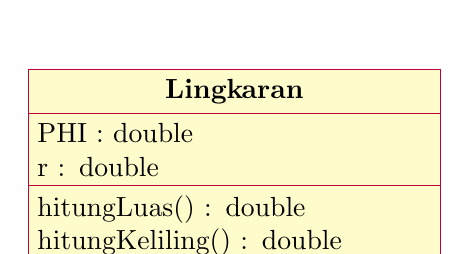
\begin{tikzpicture}
            \begin{class}[text width=5cm]{Lingkaran}{0,0}
                \attribute{PHI : double}
                \attribute{r : double}
                \operation{hitungLuas() : double}
                \operation{hitungKeliling() : double}
            \end{class}
        \end{tikzpicture}

        Note:
        \begin{itemize}
            \item Method \texttt{hitungLuas()} will calculate the area of the the circle
            \item Method \texttt{hitungKeliling()} will calculate the surrounding of the circle
        \end{itemize}

        \begin{minted}[autogobble,fontsize=\small]{java}
            public class Lingkaran {
                public double PHI;
                public double r;

                public double hitungLuas() {
                    return PHI * r * r;
                }

                public double hitungKeliling() {
                    return PHI * r * 2;
                }
            }
        \end{minted}
    }
    \item {
        In the video game rental and shop, the most important data that they manage is \textbf{RentalTransaction}.
        It contains \texttt{memberId}, \texttt{memberName}, \texttt{gameName}, \texttt{dailyPrice}, and \texttt{dayRent} (how many days it will be rent).
        It has a method to print the rental data and the price that should be paid by member. Please create a class diagram of the class and make the code.

        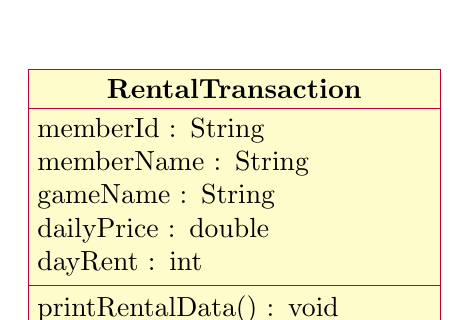
\begin{tikzpicture}
            \begin{class}[text width=5cm]{RentalTransaction}{0,0}
                \attribute{memberId : String}
                \attribute{memberName : String}
                \attribute{gameName : String}
                \attribute{dailyPrice : double}
                \attribute{dayRent : int}
                \operation{printRentalData() : void}
            \end{class}
        \end{tikzpicture}

        \newpage

        \begin{minted}[autogobble,fontsize=\small]{java}
            class RentalTransaction {
                public String memberId;
                public String memberName;
                public String gameName;
                public double dailyPrice;
                public int dayRent;

                public RentalTransaction(
                    String memberId,
                    String memberName,
                    String gameName,
                    double dailyPrice,
                    int dayRent
                ) {
                    this.memberId = memberId;
                    this.memberName = memberName;
                    this.gameName = gameName;
                    this.dailyPrice = dailyPrice;
                    this.dayRent = dayRent;
                }

                void printRentalData() {
                    System.out.printf("Member ID: %s\n", memberId);
                    System.out.printf("Member Name: %s\n", memberName);
                    System.out.printf("Game Name: %s\n", gameName);
                    System.out.printf("Daily Price: %.2f\n", dailyPrice);
                    System.out.printf("Day Rent: %.2f\n", dayRent);
                    System.out.print("--------------\n");
                    System.out.printf("Total Price: %.2f\n", dailyPrice * dayRent);
                }
            }
        \end{minted}
    }
    \item {
        Implement the code of this class diagram!

        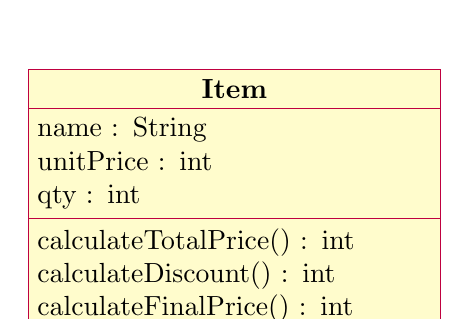
\begin{tikzpicture}
            \begin{class}[text width=5cm]{Item}{0,0}
                \attribute{name : String}
                \attribute{unitPrice : int}
                \attribute{qty : int}
                \operation{calculateTotalPrice() : int}
                \operation{calculateDiscount() : int}
                \operation{calculateFinalPrice() : int}
            \end{class}
        \end{tikzpicture}

        \begin{itemize}
            \item Method \texttt{calculateTotalPrice()} will multiply the quantity of item and the unit price
            \item {
                Method \texttt{calculateDiscount()} will calculate the discount, with the role:

                \begin{itemize}
                    \item If total $price > 100.000$, the discount will be 10\%
                    \item If the total price between $50.000 - 100.000$, the discount price will be 5\%
                    \item Method \texttt{calculateFinalPrice()} will calculate the price should be paid (total price minus discount)
                \end{itemize}
            }
        \end{itemize}

        \begin{minted}[autogobble,fontsize=\small]{java}
            public class Item {
                public String name;
                public int unitPrice;
                public int qty;

                public Item(String name, int unitPrice, int qty) {
                    this.name = name;
                    this.unitPrice = unitPrice;
                    this.qty = qty;
                }

                public int calculateTotalPrice() {
                    return unitPrice * qty;
                }

                public int calculateDiscount() {
                    int totalPrice = calculateTotalPrice();
                    if (totalPrice > 100_000) return totalPrice * 0.1;
                    if (totalPrice > 50_000) return totalPrice * 0.05;
                    return 0;
                }

                public int calculateFinalPrice() {
                    int totalPrice = calculateTotalPrice();
                    int discount = calculateDiscount();
                    return totalPrice - discount;
                }
            }
        \end{minted}
    }
    \item {
        Implement the code of class diagram below

        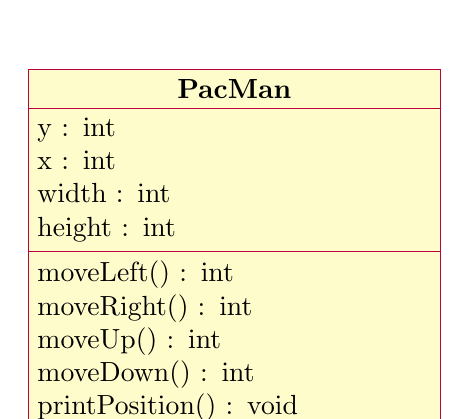
\begin{tikzpicture}
            \begin{class}[text width=5cm]{PacMan}{0,0}
                \attribute{y : int}
                \attribute{x : int}
                \attribute{width : int}
                \attribute{height : int}
                \operation{moveLeft() : int}
                \operation{moveRight() : int}
                \operation{moveUp() : int}
                \operation{moveDown() : int}
                \operation{printPosition() : void}
            \end{class}
        \end{tikzpicture}

        \begin{itemize}
            \item Attribute \texttt{x} depicts the horizontal position/coordinate of Pacman, while attribute \texttt{y} depicts the vertical coordinate
            \item Attribute \texttt{width} is for canvas width, and attribute \texttt{height} is for the height of the canvas
            \item {
                Method \texttt{moveLeft()} will move Pacman to the left (coordinate x will decrease),
                while \texttt{moveRight()} will move Pacman to the right (coordinate x will increase).
                The value of x will range from 0 to width value
            }
            \item {
                Method \texttt{moveUp()} will move Pacman to the upper position (coordinate y will decrease),
                while \texttt{moveDown()} will move Pacman to the lower position (coordinate y will increase).
                The value of y must be between 0 to height value
            }
        \end{itemize}

        \newpage

        \begin{minted}[autogobble,fontsize=\small]{java}
            public class Pacman {
                public int x;
                public int y;
                public int width;
                public int height;

                public int moveLeft() {
                    int movedValue = x - 1;
                    if (movedValue >= 0) {
                        x = movedValue;
                    }
                    return x; 
                }

                public int moveRight() {
                    int movedValue = x + 1;
                    if (movedValue <= width) {
                        x = movedValue;
                    }
                    return x;
                }

                public int moveUp() {
                    int movedValue = y - 1;
                    if (movedValue >= 0) {
                        y = movedValue;
                    }
                    return y; 
                }

                public int moveDown() {
                    int movedValue = y + 1;
                    if (movedValue <= height) {
                        y = movedValue;
                    }
                    return y;
                }

                public void printPosition() {
                    System.out.println("Position X: " + x);
                    System.out.println("Position Y: " + y);
                }
            }
        \end{minted}
    }
\end{enumerate}

\end{document}

